% ============================================================================
\section{Introduction}
\label{sec:introduction}
% ============================================================================

Electrification is pushing traction-drive propulsion and fast-charging
power toward several hundred kilowatts, while system-level performance
requirements continue to rise \cite{EVTractionReview2023}. Increasing
the dc-link voltage has emerged as a primary design lever for meeting
both demands. On the propulsion side, a higher dc-link voltage
improves efficiency and power density \cite{DriveCodesign800V2023}. On
the battery and charging side, it reduces the current required for a
given power level, lowering cable conduction loss and conductor
cross-section while enabling higher charging power under a given
current limit \cite{Post800V2026}.

This trend, however, is not without consequence at the converter
level. A higher dc-link voltage also brings more severe
insulation-coordination and electromagnetic-compatibility (EMC)
demands, together with added thermal and reliability stress on the
power stage \cite{DriveCodesign800V2023,Post800V2026}.
Fig.~\ref{fig:intro_hv_motivation} summarizes this qualitative
tradeoff between a conventional low-voltage and a higher-voltage
traction architecture. Raising the dc-link voltage therefore does not
amount to a simple rescaling of an existing inverter design; it
reshapes the architecture-level design space of the complete electric
drive.


\begin{figure}[!t]
\centering
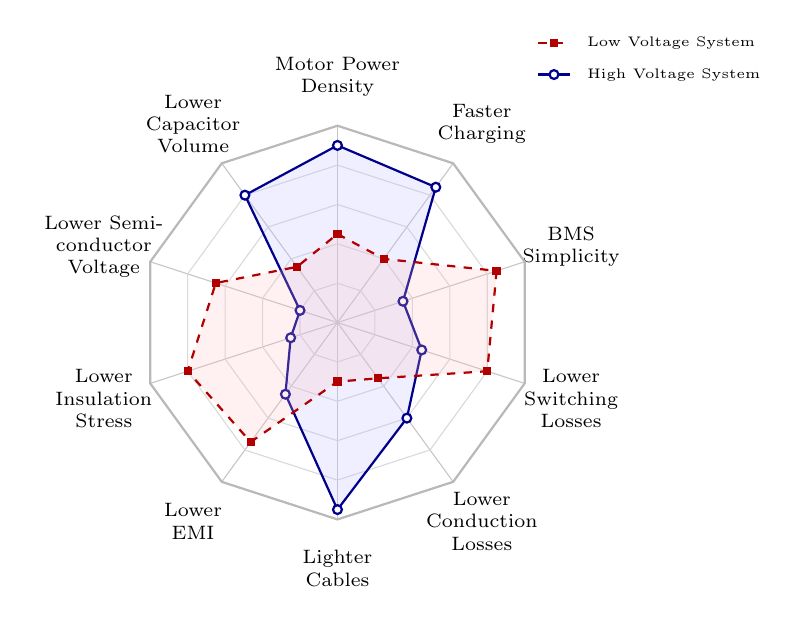
\begin{tikzpicture}[font=\scriptsize,>=latex]
\def\R{2.5}
% illustrative, qualitative per-axis extent (not measured/simulated data)
% axis order (i=0..9, angle=90-i*36): Motor Power Density, Faster
% Charging, BMS Simplicity, Lower Switching Losses, Lower Conduction
% Losses, Lighter Cables, Lower EMI, Lower Insulation Stress, Lower
% Semiconductor Voltage, Lower Capacitor Volume
\foreach \i/\lab in {0/{Motor Power\\Density},1/{Faster\\Charging},
  2/{BMS\\Simplicity},3/{Lower Switching\\Losses},
  4/{Lower Conduction\\Losses},5/{Lighter\\Cables},6/{Lower\\EMI},
  7/{Lower Insulation\\Stress},8/{Lower Semiconductor\\Voltage},
  9/{Lower Capacitor\\Volume}}{
  \pgfmathsetmacro{\ang}{90-\i*36}
  \draw[gray!45,thin] (0,0) -- (\ang:\R);
  \node[align=center,text width=17mm] at (\ang:\R+0.62) {\lab};
}
\foreach \rr in {0.5,1.0,1.5,2.0,2.5}{
  \draw[gray!30,thin] (90:\rr) \foreach \i in {1,...,9}{
    -- (90-\i*36:\rr)
  } -- cycle;
}
\draw[gray!55,thick] (90:\R) \foreach \i in {1,...,9}{
  -- (90-\i*36:\R)
} -- cycle;
% High-voltage system (blue, solid, open circle markers)
\draw[blue!55!black,thick,fill=blue!25,fill opacity=0.25]
  (90:0.90*\R) -- (54:0.85*\R) -- (18:0.35*\R) -- (-18:0.45*\R)
  -- (-54:0.60*\R) -- (-90:0.95*\R) -- (-126:0.45*\R)
  -- (-162:0.25*\R) -- (162:0.20*\R) -- (126:0.80*\R) -- cycle;
\foreach \ang/\v in {90/0.90,54/0.85,18/0.35,-18/0.45,-54/0.60,
  -90/0.95,-126/0.45,-162/0.25,162/0.20,126/0.80}{
  \node[draw=blue!55!black,fill=white,circle,thick,
    minimum size=3.2pt,inner sep=0pt] at (\ang:\v*\R) {};
}
% Low-voltage system (red, dashed, filled square markers)
\draw[red!70!black,thick,dashed,fill=red!25,fill opacity=0.22]
  (90:0.45*\R) -- (54:0.40*\R) -- (18:0.85*\R) -- (-18:0.80*\R)
  -- (-54:0.35*\R) -- (-90:0.30*\R) -- (-126:0.75*\R)
  -- (-162:0.80*\R) -- (162:0.65*\R) -- (126:0.35*\R) -- cycle;
\foreach \ang/\v in {90/0.45,54/0.40,18/0.85,-18/0.80,-54/0.35,
  -90/0.30,-126/0.75,-162/0.80,162/0.65,126/0.35}{
  \node[draw=red!70!black,fill=red!70!black,
    minimum width=2.6pt,minimum height=2.6pt,inner sep=0pt]
    at (\ang:\v*\R) {};
}
% Legend, upper right, line+marker style
\draw[red!70!black,thick,dashed] (2.55,3.55) -- (2.95,3.55);
\node[draw=red!70!black,fill=red!70!black,minimum width=2.6pt,
  minimum height=2.6pt,inner sep=0pt] at (2.75,3.55) {};
\node[anchor=west,font=\tiny] at (3.05,3.55) {Low Voltage System};
\draw[blue!55!black,thick] (2.55,3.15) -- (2.95,3.15);
\node[draw=blue!55!black,fill=white,circle,thick,minimum size=3.2pt,
  inner sep=0pt] at (2.75,3.15) {};
\node[anchor=west,font=\tiny] at (3.05,3.15) {High Voltage System};
\end{tikzpicture}
\caption{Conceptual illustration of the qualitative system-level
tradeoffs between a low-voltage and a high-voltage traction
architecture.}
\label{fig:intro_hv_motivation}
\end{figure}

\subsection{Literature and Industry Trends Toward Higher DC-Link Voltage}

The trend motivated above is not merely conceptual: it is already
established in academic prototypes, industrial inverter platforms, and
production vehicles, as summarized in
Table~\ref{tab:intro_voltage_power}. Reported academic demonstrators
range from 400-V to 800-V and 1.2-kV converters, with still higher
levels investigated for high-power passenger and heavy-duty
applications \cite{Post800V2026}, while industrial platforms
increasingly target 800-V operation as a baseline and production
vehicles show a comparable shift from established 400-V architectures
to a growing number of 800-V and higher-voltage platforms
\cite{Aghabali2021TTE800V,Mousavi2025ICTEM800V}. This industry-wide
direction, rather than an isolated research interest, motivates the
semiconductor-level analysis that follows since the rising dc-link voltages
translate directly into a semiconductor-level bottleneck.

\begin{table*}[!t]
\caption{Representative voltage and power levels in published
traction-inverter studies, industrial and reference platforms, and
production battery-electric vehicles. }
\label{tab:intro_voltage_power}
\centering
\footnotesize
\renewcommand{\arraystretch}{1.18}
\setlength{\tabcolsep}{6pt}

\begin{tabular}{
p{0.25\textwidth}
p{0.32\textwidth}
p{0.36\textwidth}}
\hline

\multicolumn{1}{l}{\textbf{Published studies / demonstrators}} &
\multicolumn{1}{l}{\textbf{Industrial / reference platforms}} &
\multicolumn{1}{l}{\textbf{Production vehicles}} \\

\hline

\textbf{Bertelshofer et al.}:
400~V, 150~kW
\cite{Bertelshofer2019SiC150kW}
&
\textbf{Bosch Gen.~4}:400/800~V, 250/350~kW
\cite{BoschInverterGen4}
&
\textbf{BMW i4 M50}:
400~V, 400~kW
\cite{BMWi4M50Specifications}
\\

\textbf{Taha et al.}:
800~V, 100~kW
\cite{Taha2024SixPhase100kW}
&
\textbf{Wolfspeed reference design}:
800~V, 300~kW
\cite{TIWolfspeed300kW}
&
\textbf{Hyundai IONIQ 5 N}:
800~V, 478~kW
\cite{HyundaiIoniq5N2026}
\\

\textbf{Al-Hmoud et al.}:
1~kV, 200~kW
\cite{AlHmoud2023Traction}
&
\textbf{Infineon eCAV platform}:
800~V, 250~kW
\cite{InfineonCAV250kW}
&
\textbf{Volvo EX90 Performance}:
800~V, 500~kW
\cite{VolvoEX90Specifications2026}
\\

\textbf{Wang et al.}:
1.2~kV, 100~kW
\cite{Wang2021ANPC1200V}
&
\textbf{AVL PI850e}:
800~V, 250~kW
\cite{AVLPI850e}
&
\textbf{Porsche Taycan Turbo S}:
800~V, 700~kW
\cite{PorscheTaycanTurboS2026}
\\

\textbf{Ayaz et al.}:
1.2~kV, 250~kW
\cite{TwoLevel_Enes}
&
\textbf{Punch IV5}:
800~V, 600~kW
\cite{PunchIV5}
&
\textbf{Lucid Air Dream Performance}:
900~V, 828~kW
\cite{LucidAirDreamPerformance}
\\

\hline
\end{tabular}
\end{table*}

\subsection{Semiconductor Blocking-Voltage Tradeoff}

\label{sec:semiconductor_limitations}

In a conventional two-level voltage-source inverter, each active
switch must block a voltage directly tied to the complete dc-link
voltage. In unipolar power devices, a higher blocking-voltage rating
imposes a fundamental tradeoff against both specific on-state
resistance and switching performance, commonly captured by the figure
of merit, as shown in Fig.~\ref{fig:intro_ronsp_trend}
\cite{Millan2014WBGSurvey,SpecificResistance}. Therefore, a lower-voltage device
consistently achieves a higher FOM than a higher-voltage device of the
same material.

\begin{figure}[!t]
\centering
\resizebox{\columnwidth}{!}{%
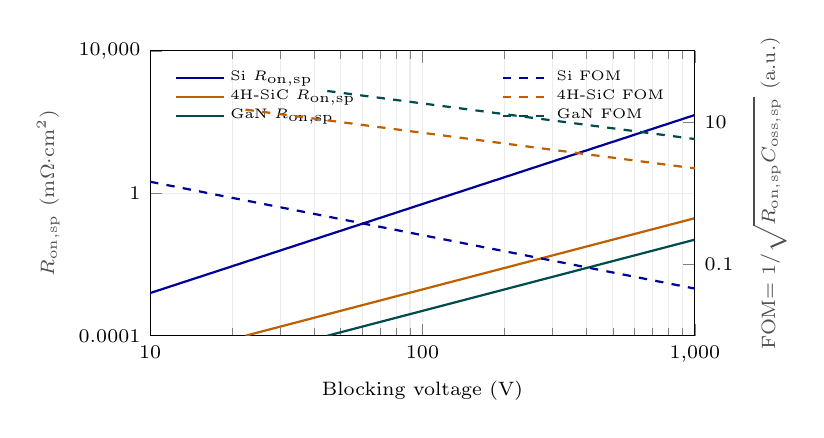
\begin{tikzpicture}
\begin{axis}[
    width=8.5cm,
    height=52mm,
    font=\scriptsize,
    xlabel={Blocking voltage (V)},
    ylabel={$R_{\mathrm{on,sp}}$ (m$\Omega\cdot$cm$^2$)},
    xmode=log, ymode=log,
    log ticks with fixed point,
    xmin=10,xmax=1000,
    ymin=1e-4,ymax=1e4,
    tick label style={font=\scriptsize},
    xlabel style={font=\scriptsize},
    ylabel style={font=\scriptsize,black!70},
    axis y line*=left,
    grid=both,
    grid style={gray!15},
    legend style={font=\tiny,draw=none,fill=none,
      at={(0.03,0.97)},anchor=north west,row sep=-2pt},
    legend cell align=left,
]
\addplot[blue!60!black,thick,solid,domain=10:1000,samples=60] {5e-6*x^2.5};
\addlegendentry{Si $R_{\mathrm{on,sp}}$}
\addplot[orange!75!black,thick,solid,domain=22.4:1000,samples=60] {2e-7*x^2};
\addlegendentry{4H-SiC $R_{\mathrm{on,sp}}$}
\addplot[teal!60!black,thick,solid,domain=44.7:1000,samples=60] {5e-8*x^2};
\addlegendentry{GaN $R_{\mathrm{on,sp}}$}
\end{axis}
\begin{axis}[
    width=8.5cm,
    height=52mm,
    font=\scriptsize,
    xmode=log, ymode=log,
    log ticks with fixed point,
    xmin=10,xmax=1000,
    ymin=1e-2,ymax=1e2,
    axis y line*=right,
    axis x line=none,
    ylabel={FOM$=1/\sqrt{R_{\mathrm{on,sp}}C_{\mathrm{oss,sp}}}$ (a.u.)},
    ylabel style={font=\scriptsize,black!70},
    tick label style={font=\scriptsize},
    legend style={font=\tiny,draw=none,fill=none,
      at={(0.97,0.97)},anchor=north east,row sep=-2pt},
    legend cell align=left,
]
\addplot[blue!60!black,thick,dashed,domain=10:1000,samples=60] {8.17*x^(-0.75)};
\addlegendentry{Si FOM}
\addplot[orange!75!black,thick,dashed,domain=22.4:1000,samples=60] {70.7*x^(-0.5)};
\addlegendentry{4H-SiC FOM}
\addplot[teal!60!black,thick,dashed,domain=44.7:1000,samples=60] {182.6*x^(-0.5)};
\addlegendentry{GaN FOM}
\end{axis}
\end{tikzpicture}}
    \caption{Ideal one-dimensional unipolar specific on-state
    resistance $R_{\mathrm{on,sp}}$ (left axis, solid) and the
    resulting high-frequency figure of merit
    $\mathrm{FOM}=1/\sqrt{R_{\mathrm{on,sp}}C_{\mathrm{oss,sp}}}$
    (right axis, dashed, arbitrary units) versus blocking voltage for
    Si, 4H-SiC, and GaN.}
    \label{fig:intro_ronsp_trend}
\end{figure}

Wide-bandgap (WBG) semiconductors shift this FOM favorably: SiC
metal-oxide-semiconductor field-effect transistors (MOSFETs) now
dominate high-voltage automotive drives, while GaN is particularly
attractive at lower voltage owing to its fast switching behavior and
superior FOM \cite{WideReview2018,WBGTractionReview2025,GaNComparison,
Millan2014WBGSurvey}. 
Yet switching material does not remove the
underlying coupling between dc-link voltage and device voltage class:
irrespective of technology, a higher dc-link voltage still forces a
higher-voltage, higher-$R_{\mathrm{on,sp}}$ device and higher swithcing losses. 
Converter architectures that partition the dc-link voltage among multiple
switching units, so each device blocks only a fraction of the total
voltage, therefore become increasingly relevant as system voltage
rises.

\subsection{Multilevel Converters and Their Limitations}

Multilevel converters constitute an established solution to this
voltage-partitioning problem.
NPC, T-type, flying-capacitor, and cascaded architectures all distribute
the dc-link voltage among
additional semiconductor positions or capacitor-voltage levels,
reducing individual device voltage stress
\cite{Poorfakhraei2021MultilevelReview,T_type_SiC,
FlyingCap_Optimized3D,CascadedHBridge_control}.

This voltage partitioning, however, comes at the cost of additional
semiconductor devices, passive components, and gate drivers -- each an
additional potential failure point -- without, by itself, yielding a
modular converter--machine system: because the added semiconductor
positions continue to feed a single, electrically common three-phase
winding set, a fault at one position cannot generally be isolated and
bypassed without disabling the drive.
 Fault tolerance, power
redistribution, and post-fault reconfiguration can be implemented in
conventional multilevel drives, but typically require additional
redundancy, dedicated isolation paths, and specialized control layered
on top of the base topology rather than following from it. A larger
semiconductor count therefore does not yield a commensurate increase
in fault tolerance, motivating an alternative form of voltage
partitioning.

\subsection{Stacked Polyphase Bridge}
\label{sec:spb_modularity}

Unlike other multilevel converters, which distribute the dc-link
voltage among additional semiconductor positions within a single
converter, the stacked polyphase bridge (SPB) distributes the
high-voltage conversion function among $N$ repeated converter units.
Each unit is a conventional three-phase two-level bridge connected in
series on the dc side, supplying its own electrically separated
three-phase winding group of the same machine, as illustrated in
Fig.~\ref{fig:spb_architecture}.

Under balanced operation, each cell's local dc-link voltage
$V_{\mathrm{dc},k}\approx V_{\mathrm{dc}}/N$, so the semiconductor
voltage rating can be selected on the local cell voltage rather than
the complete traction dc-link voltage -- addressing the semiconductor
bottleneck much as multilevel converters do. Because each cell also
drives its own separated winding group, however, SPB additionally has
an inherently modular structure that multilevel converters lack: a
faulted cell can, in principle, be isolated and bypassed while the
remaining cells continue to drive the machine at reduced power. It is
this combination of semiconductor voltage reduction and
converter--machine modularity that distinguishes SPB from conventional
multilevel and cascaded architectures and motivates its consideration
as a candidate topology for next-generation traction drives.

\begin{figure}[!t]
\centering
\resizebox{0.72\columnwidth}{!}{%
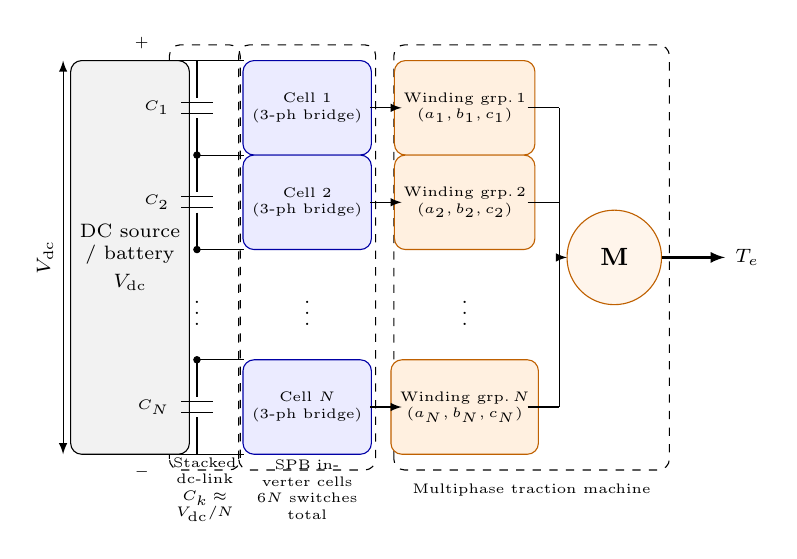
\begin{tikzpicture}[font=\scriptsize,>=latex,x=1mm,y=1mm]
% ---- styles ----
\tikzstyle{src}=[draw,rounded corners,align=center,fill=gray!10,
  minimum width=9mm,minimum height=50mm]
\tikzstyle{cellbox}=[draw=blue!65!black,rounded corners,align=center,
  fill=blue!8,minimum width=16mm,minimum height=12mm,font=\tiny]
\tikzstyle{windbox}=[draw=orange!75!black,rounded corners,align=center,
  fill=orange!12,minimum width=16mm,minimum height=12mm,font=\tiny]

% ---- group boxes (drawn first, underneath) ----
\draw[dashed,rounded corners] (9.5,-27) rectangle (18.5,27);
\draw[dashed,rounded corners] (18.3,-27) rectangle (35.7,27);
\draw[dashed,rounded corners] (38,-27) rectangle (73,27);

% ---- under-box labels ----
\node[font=\tiny,align=center,text width=9mm] at (14,-29.5)
  {Stacked dc-link\\$C_k\!\approx\!V_{\mathrm{dc}}/N$};
\node[font=\tiny,align=center,text width=17mm] at (27,-29.5)
  {SPB inverter cells\\$6N$ switches total};
\node[font=\tiny,align=center] at (55.5,-29.5)
  {Multiphase traction machine};

% ---- DC source ----
\node[src] (src) at (4.5,0) {DC source\\/ battery\\[2pt]$V_{\mathrm{dc}}$};
\draw[<->] (-4,-25) -- (-4,25);
\node[rotate=90] at (-6.3,0) {$V_{\mathrm{dc}}$};
\node[font=\tiny,anchor=south] at (6,25.3) {$+$};
\node[font=\tiny,anchor=north] at (6,-25.3) {$-$};

% ---- rails ----
\draw (9,25) -- (19,25);
\draw (9,-25) -- (19,-25);

% ---- stacked dc-link chain ----
\draw (13,25) -- (13,20.3);
\draw (11,19.7) -- (15,19.7);
\draw (11,18.3) -- (15,18.3);
\draw (13,17.7) -- (13,13);
\filldraw (13,13) circle (0.4);
\draw (13,13) -- (19,13);
\node[font=\tiny,anchor=east] at (10.7,19) {$C_1$};

\draw (13,13) -- (13,8.3);
\draw (11,7.7) -- (15,7.7);
\draw (11,6.3) -- (15,6.3);
\draw (13,5.7) -- (13,1);
\filldraw (13,1) circle (0.4);
\draw (13,1) -- (19,1);
\node[font=\tiny,anchor=east] at (10.7,7) {$C_2$};

\node[font=\scriptsize] at (13,-6) {$\vdots$};

\filldraw (13,-13) circle (0.4);
\draw (13,-13) -- (19,-13);
\draw (13,-13) -- (13,-17.7);
\draw (11,-18.3) -- (15,-18.3);
\draw (11,-19.7) -- (15,-19.7);
\draw (13,-20.3) -- (13,-25);
\node[font=\tiny,anchor=east] at (10.7,-19) {$C_N$};

% ---- SPB bridge cells ----
\node[cellbox] (c1) at (27,19) {Cell 1\\(3-ph bridge)};
\node[cellbox] (c2) at (27,7) {Cell 2\\(3-ph bridge)};
\node[font=\scriptsize] at (27,-6) {$\vdots$};
\node[cellbox] (cN) at (27,-19) {Cell $N$\\(3-ph bridge)};

% ---- winding groups ----
\node[windbox] (w1) at (47,19) {Winding grp.\,1\\$(a_1,b_1,c_1)$};
\node[windbox] (w2) at (47,7) {Winding grp.\,2\\$(a_2,b_2,c_2)$};
\node[font=\scriptsize] at (47,-6) {$\vdots$};
\node[windbox] (wN) at (47,-19) {Winding grp.\,$N$\\$(a_N,b_N,c_N)$};

\draw[->] (35,19) -- (39,19);
\draw[->] (35,7) -- (39,7);
\draw[->] (35,-19) -- (39,-19);

% ---- bus to machine ----
\draw (55,19) -- (59,19);
\draw (55,7) -- (59,7);
\draw (55,-19) -- (59,-19);
\draw (59,19) -- (59,-19);
\draw[->] (59,0) -- (60,0);

% ---- machine ----
\node[circle,draw=orange!75!black,fill=orange!8,minimum size=12mm,
  font=\bfseries\small] (M) at (66,0) {M};
\draw[->,thick] (M.east) -- ++(8,0) node[right,font=\scriptsize] {$T_e$};

\end{tikzpicture}}
    \caption{Conceptual architecture of an $N$-cell SPB traction
    drive. The dc source $V_{\mathrm{dc}}$ feeds $N$ series-connected
    local dc-link capacitors, each nominally $V_{\mathrm{dc}}/N$, that
    individually supply $N$ series-connected three-phase two-level
    bridge cells ($6N$ switches total); each cell drives one
    electrically separated three-phase winding group of the same
    machine, and the combined winding groups produce the
    electromagnetic torque $T_e$.}
    \label{fig:spb_architecture}
\end{figure}

SPB was introduced by Norrga \textit{et al.} for compact EV and HEV
drives \cite{Norrga2013SPB}; its subsequent development toward
higher-fidelity control, balancing, and reconfiguration is traced in
detail in Section~\ref{sec:evolution}.

Realizing this potential, however, introduces its own design
challenges: component count, dc-link dynamics, machine design,
common-mode voltage and insulation coordination, and fault handling
all become more tightly coupled, as examined in the sections that
follow, with thermal management identified as an open research
direction (Section~\ref{sec:future_directions}).

These questions have grown more relevant as neighboring research
areas have matured: multiphase machines provide additional
post-fault degrees of freedom, integrated modular motor drives show
how repeated power-electronic units can be physically associated with
individual machine sections, wide-bandgap semiconductors amplify
performance differences among voltage classes, and distributed
control coordinates modular converter units
\cite{Choi2011IMMD,Wang2025GaNIMMD,
JahnsDai2017IMDReview,Bringezu2020SPB,Deng2026IMDReview,
Ebrahimian2025GaNIMMD} -- together motivating SPB's assessment as a
complete converter--machine architecture rather than only a
series-connected topology.

Despite more than a decade of research on SPB, however, no study has
yet brought these threads together to systematically assess its
feasibility for electric-vehicle traction applications. The available
literature remains distributed across converter topology, modulation,
dc-link stability, multiphase-machine design, integrated motor drives,
semiconductor technology, thermal management, distributed control, and
fault-tolerant operation. Although these topics are strongly coupled
in an SPB traction drive, they are rarely evaluated within a common
system boundary. Moreover, most reported SPB experimental
demonstrations remain validated only at laboratory scale
(Section~\ref{sec:evolution}), even as the enabling
semiconductor, machine, cooling, and packaging technologies continue
to advance rapidly. This gap between a well-motivated architectural
concept and a system-level feasibility assessment is the gap that the
present paper addresses.

Accordingly, this paper provides a system-level review of SPB
traction-drive technology aimed at closing that gap. The remainder of
the paper is organized as follows. First, the historical development,
operating principle, and modulation of SPB are consolidated. Second,
the interaction between SPB cell count and the electric machine is
examined together with relevant multiphase-machine and integrated
modular motor-drive research, including the physical-integration and
insulation-coordination overhead introduced by series-connected
converter cells. Third, the series-stack origin of common-mode voltage
in SPB, its physical consequences, and mitigation options are
examined, followed by dc-link dynamics and balancing. Fourth,
semiconductor voltage scaling, SiC and GaN device selection, loss
scaling, and fault handling and reconfiguration are considered as
coupled architecture-level design problems. Finally, the research gaps
and requirements for high-power automotive validation are identified,
including high-power EMC validation and the quantitative comparison
against conventional two-level, multilevel, and cascaded alternatives
that remain open for future work.